\begin{usecase}{Create Calendar}
  \ucbasicinfo{High}{Regular}
  \ucshortdescription{This UC allows the user to create a new calendar using iOS EventKit.}
  \uctrigger{This UC is triggered when the user clicks ``Create Calendar'' in the app.}
  \ucactors{User}{EventKit}
  \ucpreconditions{
    \begin{itemize}
      \item User must be logged in
      \item Calendar access must be authorized in iOS Settings
      \item Baikal CalDAV account must be configured
    \end{itemize}
  }
  \ucrelationships{N/A}{N/A}{N/A}
  \ucinputsoutputs{
    \begin{itemize}
      \item \textbf{Calendar name} (Source: User)
      \item \textbf{Calendar account to add calendar under} (Source: User)
      \item \textbf{Calendar color} (Source: User)
    \end{itemize}
  }{
    \begin{itemize}
      \item \textbf{New calendar} (Destination: EventKit)
      \item \textbf{Creation status} (Destination: App)
    \end{itemize}
  }
  \ucmainflow{
    \begin{enumerate}
      \item The user taps the ``Calendar'' icon button in the app toolbar in the ``Calendar'' screen.
            \ucinfo{The app presents a ``Calendars'' sheet.}
      \item The user clicks the ``plus'' icon button in the toolbar of the ``Calendars'' sheet.
            \ucinfo{The app presents a form for calendar name, selector to choose account to add calendar under, and calendar color.}
      \item The user enters calendar name, selects a color, and selector to choose account to add calender under.
            \ucinfo{The app uses EventKit to create a new calendar.}
      \item EventKit creates the calendar and handles synchronization.
            \ucinfo{The calendar appears in the user's calendar list.}
    \end{enumerate}
  }
  \ucalternateflows{
    \begin{itemize}
      \item If calendar creation fails, the app shows an error and allows retry.
    \end{itemize}
  }
  \ucexceptions{
    \begin{itemize}
      \item \textbf{EventKit access denied:} The app prompts to enable calendar access in Settings.
      \item \textbf{Network issues:} EventKit handles synchronization internally.
    \end{itemize}
  }
  \ucconclusion{The UC ends when EventKit confirms the calendar creation.}
  \ucpostconditions{A new calendar is created through EventKit.}
  \ucspecialrequirements{The system must use EventKit for all calendar operations.}
\end{usecase}

\begin{figure}[!h]
  \centering
  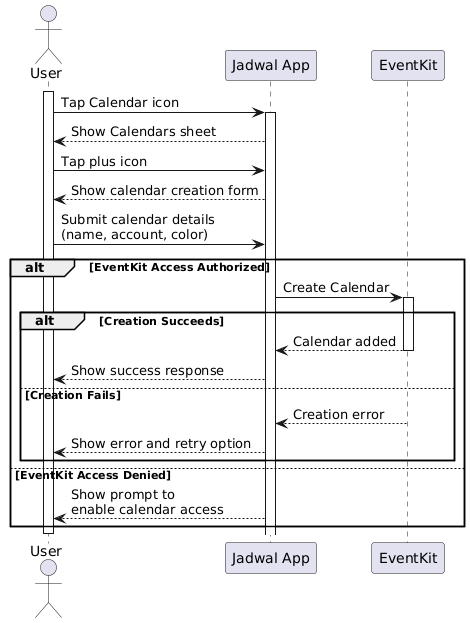
\includegraphics[width=0.5\textwidth]{images/docs/diagrams/sequence-diagrams/all-sequence-diagrams/Create Calendar.png}
  \caption{Create Calendar Sequence Diagram}
  \label{fig:seq/create-calendar}
\end{figure}

The ``Create Calendar Sequence Diagram'', shown in \textbf{Figure~\ref{fig:seq/create-calendar}}, illustrates the process of creating a new calendar in the Jadwal app. The sequence begins when the user accesses the calendar creation interface through the ``Calendars'' sheet, accessed via the calendar icon in the toolbar.

The flow involves several key steps:
\begin{enumerate}
  \item The user provides essential calendar details through a form interface:
        \begin{itemize}
          \item Calendar name
          \item Account selection (where to add the calendar)
          \item Calendar color
        \end{itemize}
  \item The app communicates with EventKit to create the new calendar
  \item EventKit handles the calendar creation and all necessary synchronization
\end{enumerate}

The process is designed to be robust and user-friendly:
\begin{itemize}
  \item If EventKit access is denied, the app guides users to enable calendar access in iOS Settings
  \item If creation fails, the app shows an error and allows retry
  \item EventKit handles all synchronization internally
\end{itemize}

This implementation leverages iOS's native EventKit framework, which manages all calendar operations and synchronization internally. This provides a reliable and native iOS experience while ensuring proper calendar management.